\chapter{Linked Data Structures}

\textbf{Readings:} CP:AMA 17.5--17.6.

\tikzset{
  lnode/.style={draw,rectangle split,rectangle split parts=2,rectangle split horizontal,
    minimum height=0.7cm,inner sep=4pt},
  ptr/.style={-{Stealth[length=2mm]},thick}
}

\section{Linked Lists}

Racket lists are \emph{linked}: each \code{cons} holds an item and a reference to the rest of
the list. In C we build them ourselves with a self-referential structure:
\begin{lstlisting}[style=c]
struct llnode {
  int item;
  struct llnode *next;    // NULL marks the end of the list
};
\end{lstlisting}
A structure cannot contain itself, but it can contain a \emph{pointer} to its own type.
\begin{center}
\begin{tikzpicture}
  \node (lst) {\code{lst}};
  \node[lnode,right=1cm of lst] (a) {12 \nodepart{two} \phantom{x}};
  \node[lnode,right=1cm of a] (b) {5 \nodepart{two} \phantom{x}};
  \node[lnode,right=1cm of b] (c) {9 \nodepart{two} \phantom{x}};
  \node[right=1cm of c] (n) {\code{NULL}};
  \draw[ptr] (lst) -- (a);
  \draw[ptr] (a.two east) ++(-0.2,0) -- (b);
  \draw[ptr] (b.two east) ++(-0.2,0) -- (c);
  \draw[ptr] (c.two east) ++(-0.2,0) -- (n);
\end{tikzpicture}
\end{center}

\subsection{Building lists}
\begin{lstlisting}[style=c]
// cons(first, rest) produces a new node with item first, followed by rest
// effects: allocates memory (caller must free, e.g. with list_destroy)
// time: O(1)
struct llnode *cons(int first, struct llnode *rest) {
  struct llnode *new = malloc(sizeof(struct llnode));
  new->item = first;
  new->next = rest;
  return new;
}

struct llnode *lst = cons(12, cons(5, cons(9, NULL)));
\end{lstlisting}

\subsection{Traversal}

Linked lists can be traversed recursively (like Racket) or iteratively:
\begin{lstlisting}[style=c]
// length(lst) produces the number of nodes in lst
// time: O(n)
int length(const struct llnode *lst) {
  int len = 0;
  while (lst) {           // same as lst != NULL
    ++len;
    lst = lst->next;      // lst is a local copy; the list is unchanged
  }
  return len;
}

int length_rec(const struct llnode *lst) {
  if (lst == NULL) return 0;
  return 1 + length_rec(lst->next);
}

// print_list(lst) prints the items of lst
void print_list(const struct llnode *lst) {
  for (const struct llnode *node = lst; node; node = node->next) {
    printf("%d ", node->item);
  }
  printf("\n");
}
\end{lstlisting}
The iterative version uses $\bigO(1)$ stack space, whereas the recursive one uses $\bigO(n)$ and
can overflow on long lists.

\subsection{Destroying a list}
\begin{lstlisting}[style=c]
// list_destroy(lst) frees every node of lst
// time: O(n)
void list_destroy(struct llnode *lst) {
  while (lst) {
    struct llnode *next = lst->next;   // save before freeing!
    free(lst);
    lst = next;
  }
}
\end{lstlisting}
Writing \code{free(lst); lst = lst->next;} would use freed memory.

\subsection{Mutating lists}

Unlike Racket, we can change a list in place. Mapping in place:
\begin{lstlisting}[style=c]
void list_sqr(struct llnode *lst) {
  for (struct llnode *node = lst; node; node = node->next) {
    node->item *= node->item;
  }
}
\end{lstlisting}
Copying (like Racket's functional style) must allocate new nodes:
\begin{lstlisting}[style=c]
struct llnode *list_copy(const struct llnode *lst) {
  if (lst == NULL) return NULL;
  return cons(lst->item, list_copy(lst->next));
}
\end{lstlisting}

\section{A List Wrapper Structure}

Functions that add or remove the \emph{first} node need to change the caller's pointer
\code{lst}, which would require a \code{struct llnode **}. A cleaner approach is a wrapper
structure that represents the whole list:
\begin{lstlisting}[style=c]
struct llist {
  struct llnode *front;
};

struct llist *list_create(void) {
  struct llist *lst = malloc(sizeof(struct llist));
  lst->front = NULL;
  return lst;
}

// add_front(i, lst) adds i to the front of lst
// time: O(1)
void add_front(int i, struct llist *lst) {
  lst->front = cons(i, lst->front);
}
\end{lstlisting}

\subsection{Inserting into a sorted list}
\begin{lstlisting}[style=c]
// insert(i, slst) inserts i into the sorted list slst
// requires: slst is sorted in increasing order
// time: O(n)
void insert(int i, struct llist *slst) {
  if (slst->front == NULL || i < slst->front->item) {
    add_front(i, slst);                 // special case: new first node
  } else {
    struct llnode *prev = slst->front;
    while (prev->next && i > prev->next->item) {
      prev = prev->next;
    }
    prev->next = cons(i, prev->next);   // splice in after prev
  }
}
\end{lstlisting}
\begin{center}
\begin{tikzpicture}
  \node[lnode] (a) {3 \nodepart{two} \phantom{x}};
  \node[lnode,right=1.6cm of a] (b) {8 \nodepart{two} \phantom{x}};
  \node[lnode,below right=0.8cm and 0.4cm of a] (n) {5 \nodepart{two} \phantom{x}};
  \node[above=0mm of a,font=\scriptsize] {\code{prev}};
  \draw[ptr,dashed,gray] (a.two east) ++(-0.2,0) -- (b);
  \draw[ptr] (a.two south) -- (n.west);
  \draw[ptr] (n.two east) ++(-0.2,0) -- (b.south);
\end{tikzpicture}
\end{center}

\subsection{Removing a node}
\begin{lstlisting}[style=c]
// remove_item(i, lst) removes the first occurrence of i from lst
//   and produces true, or produces false if i is not in lst
// time: O(n)
bool remove_item(int i, struct llist *lst) {
  if (lst->front == NULL) return false;
  if (lst->front->item == i) {
    struct llnode *old = lst->front;
    lst->front = old->next;
    free(old);
    return true;
  }
  struct llnode *prev = lst->front;
  while (prev->next && prev->next->item != i) {
    prev = prev->next;
  }
  if (prev->next == NULL) return false;
  struct llnode *old = prev->next;
  prev->next = old->next;
  free(old);
  return true;
}
\end{lstlisting}
Removing 8 from the list 3, 8, 5: \code{prev->next} is redirected around the
old node, which is then freed.

\begin{center}
\begin{tikzpicture}
  \node[lnode] (a) {3 \nodepart{two} \phantom{x}};
  \node[lnode,right=1.4cm of a,draw=red!70!black,fill=red!8] (b) {8 \nodepart{two} \phantom{x}};
  \node[lnode,right=1.4cm of b] (c) {5 \nodepart{two} \phantom{x}};
  \node[right=1cm of c] (n) {\code{NULL}};
  \node[above=0mm of a,font=\scriptsize] {\code{prev}};
  \node[above=0mm of b,font=\scriptsize,red!70!black] {\code{old} (freed)};
  \draw[ptr,dashed,gray] (a.two east) ++(-0.2,0) -- (b);
  \draw[ptr,dashed,gray] (b.two east) ++(-0.2,0) -- (c);
  \draw[ptr] (c.two east) ++(-0.2,0) -- (n);
  \draw[ptr,blue!60!black] (a.two south) to[out=-60,in=-120] node[below,font=\scriptsize]{\code{prev->next = old->next}} (c.south);
\end{tikzpicture}
\end{center}

The pattern for both: handle the empty list and the front node as special cases, then walk a
\code{prev} pointer to the node \emph{before} the position of interest.

\section{Augmenting the Wrapper}

The wrapper can store extra information to make operations faster, as long as every function
keeps it up to date:
\begin{itemize}
  \item a \code{length} field makes \code{list\_length} $\bigO(1)$ instead of $\bigO(n)$;
  \item a \code{back} pointer to the last node makes adding to the back $\bigO(1)$.
\end{itemize}

\subsection{A queue with a linked list}
\begin{lstlisting}[style=c]
struct queue {
  struct llnode *front;
  struct llnode *back;
};

// time: O(1)
void queue_add_back(int i, struct queue *q) {
  struct llnode *node = cons(i, NULL);
  if (q->front == NULL) {
    q->front = node;
  } else {
    q->back->next = node;
  }
  q->back = node;
}

// requires: q is not empty
// time: O(1)
int queue_remove_front(struct queue *q) {
  assert(q->front);
  struct llnode *old = q->front;
  int item = old->item;
  q->front = old->next;
  if (q->front == NULL) {
    q->back = NULL;            // the queue is now empty
  }
  free(old);
  return item;
}
\end{lstlisting}

\begin{center}
\begin{tikzpicture}[fld/.style={draw,minimum width=1.5cm,minimum height=6mm,font=\scriptsize\ttfamily}]
  \node[fld] (fr) at (0,0) {front};
  \node[fld,below=0pt of fr] (bk) {back};
  \node[font=\scriptsize,above=0pt of fr] {\code{struct queue}};
  \node[lnode] (a) at (3,1.2) {4 \nodepart{two} \phantom{x}};
  \node[lnode,right=1cm of a] (b) {7 \nodepart{two} \phantom{x}};
  \node[lnode,right=1cm of b] (c) {2 \nodepart{two} \phantom{x}};
  \node[right=0.8cm of c] (n) {\code{NULL}};
  \draw[ptr] (fr.east) to[out=0,in=180] (a.west);
  \draw[ptr] (bk.east) -| (c.south);
  \draw[ptr] (a.two east) ++(-0.2,0) -- (b);
  \draw[ptr] (b.two east) ++(-0.2,0) -- (c);
  \draw[ptr] (c.two east) ++(-0.2,0) -- (n);
  \node[font=\scriptsize,anchor=north] at (a.south) {remove here};
  \node[font=\scriptsize,anchor=south] at (c.north) {add here};
\end{tikzpicture}
\end{center}
Both ends are reachable in one step, so both operations are $\bigO(1)$.

\section{Arrays vs.\ Linked Lists}

\begin{center}
\begin{tabular}{lcc}
  \toprule
  Operation & Dynamic array & Linked list \\
  \midrule
  access item $i$ & $\bigO(1)$ & $\bigO(i)$ \\
  add/remove at front & $\bigO(n)$ & $\bigO(1)$ \\
  add at back & $\bigO(1)$ amortized & $\bigO(1)$ with back pointer \\
  insert/remove in middle (given position) & $\bigO(n)$ & $\bigO(1)$ after reaching it \\
  binary search (sorted) & $\bigO(\log n)$ & not possible \\
  extra memory & unused capacity & one pointer per item \\
  \bottomrule
\end{tabular}
\end{center}

\section{Trees}

A node in a binary tree has two child pointers:
\begin{lstlisting}[style=c]
struct bstnode {
  int item;
  struct bstnode *left;
  struct bstnode *right;
};
\end{lstlisting}
In a \emph{binary search tree} (BST), every item in the left subtree is less than the node's item,
and every item in the right subtree is greater.

\begin{center}
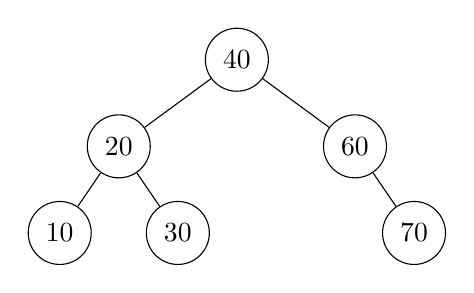
\begin{tikzpicture}[level distance=1.1cm,
  level 1/.style={sibling distance=3cm},
  level 2/.style={sibling distance=1.5cm},
  every node/.style={draw,circle,minimum size=0.8cm}]
  \node {40}
    child {node {20} child {node {10}} child {node {30}}}
    child {node {60} child[missing] child {node {70}}};
\end{tikzpicture}
\end{center}

\subsection{BST operations}
\begin{lstlisting}[style=c]
struct bst {
  struct bstnode *root;
};

// bst_find(i, t) determines if i is in t
// time: O(h), where h is the height of t
bool bst_find(int i, const struct bst *t) {
  const struct bstnode *node = t->root;
  while (node) {
    if (i == node->item) return true;
    node = (i < node->item) ? node->left : node->right;
  }
  return false;
}

static struct bstnode *new_leaf(int i) {
  struct bstnode *leaf = malloc(sizeof(struct bstnode));
  leaf->item = i;
  leaf->left = NULL;
  leaf->right = NULL;
  return leaf;
}

// bst_insert(i, t) inserts i into t (no effect if already present)
// time: O(h)
void bst_insert(int i, struct bst *t) {
  if (t->root == NULL) {
    t->root = new_leaf(i);
    return;
  }
  struct bstnode *node = t->root;
  while (true) {
    if (i == node->item) return;
    if (i < node->item) {
      if (node->left == NULL) { node->left = new_leaf(i); return; }
      node = node->left;
    } else {
      if (node->right == NULL) { node->right = new_leaf(i); return; }
      node = node->right;
    }
  }
}

// free_bstnode(node) frees every node in the subtree rooted at node
// time: O(n)
static void free_bstnode(struct bstnode *node) {
  if (node) {
    free_bstnode(node->left);
    free_bstnode(node->right);
    free(node);                    // post-order: children first
  }
}

void bst_destroy(struct bst *t) {
  free_bstnode(t->root);
  free(t);
}
\end{lstlisting}

In memory each node is a small structure with two child pointers; empty
subtrees are \code{NULL} (drawn as a slash). Inserting 25 into the tree above
follows the path $40 \to 20 \to 30$ and replaces the \code{NULL} left pointer of 30 by a
new leaf:

\begin{center}
\begin{tikzpicture}[bn/.style={draw,rectangle split,rectangle split parts=3,rectangle split horizontal,
    minimum height=6mm,inner sep=2pt,font=\small},
  bp/.style={-{Stealth[length=1.6mm]},thick}]
  \node[bn] (n40) at (0,0) {\phantom{x}\nodepart{two}40\nodepart{three}\phantom{x}};
  \node[bn] (n20) at (-3,-1.3) {\phantom{x}\nodepart{two}20\nodepart{three}\phantom{x}};
  \node[bn] (n60) at (3,-1.3) {\phantom{x}\nodepart{two}60\nodepart{three}\phantom{x}};
  \node[bn] (n10) at (-4.6,-2.6) {\phantom{x}\nodepart{two}10\nodepart{three}\phantom{x}};
  \node[bn] (n30) at (-1.4,-2.6) {\phantom{x}\nodepart{two}30\nodepart{three}\phantom{x}};
  \node[bn] (n70) at (4.4,-2.6) {\phantom{x}\nodepart{two}70\nodepart{three}\phantom{x}};
  \node[bn,fill=green!12] (n25) at (-2.6,-3.9) {\phantom{x}\nodepart{two}25\nodepart{three}\phantom{x}};
  \draw[bp] (n40.one south) -- (n20.north);
  \draw[bp] (n40.three south) -- (n60.north);
  \draw[bp] (n20.one south) -- (n10.north);
  \draw[bp,blue!60!black] (n20.three south) -- (n30.north);
  \draw[bp,green!40!black] (n30.one south) -- (n25.north);
  \draw[bp] (n60.three south) -- (n70.north);
  \foreach \n in {n60,n10,n70,n25} \draw[gray] (\n.south west) -- (\n.one split north);
  \foreach \n in {n10,n30,n70,n25} \draw[gray] (\n.two split south) -- (\n.north east);
\end{tikzpicture}
\end{center}

A recursive insert is also natural; it returns the (possibly new) root of the subtree:
\begin{lstlisting}[style=c]
static struct bstnode *insert_node(int i, struct bstnode *node) {
  if (node == NULL) return new_leaf(i);
  if (i < node->item) {
    node->left = insert_node(i, node->left);
  } else if (i > node->item) {
    node->right = insert_node(i, node->right);
  }
  return node;
}
\end{lstlisting}

\subsection{Height and balance}

BST operations are $\bigO(h)$ where $h$ is the height. A \emph{balanced} tree (e.g.\ AVL trees,
CS 240) has $h \in \bigO(\log n)$, giving $\bigO(\log n)$ operations. But inserting items in sorted
order produces a ``stick'' with $h = n$, so in the worst case BST operations are $\bigO(n)$.

\begin{aside}
Augmenting each node with the size of its subtree allows selecting the $k$-th smallest item in
$\bigO(h)$ time --- the same idea as augmenting the list wrapper with a length.
\end{aside}

\section{Graphs (briefly)}

Linked structures can also represent general graphs, where nodes may have any number of
neighbours and cycles are possible (e.g.\ an adjacency list: each node has a linked list of its
neighbours). Cycles mean traversals must remember visited nodes, and freeing must be done
carefully. Graph algorithms are covered in CS 341.

\section{Summary}
\begin{itemize}
  \item A linked list node holds an item and a \code{next} pointer; \code{NULL} ends the list.
  \item Traverse with a moving pointer; save \code{next} before \code{free}.
  \item Use a wrapper structure to handle changes to the front; augment it with length/back for
    $\bigO(1)$ operations.
  \item Arrays give fast indexing; linked lists give fast insertion/removal at known positions.
  \item BST find/insert are $\bigO(h)$: $\bigO(\log n)$ if balanced, $\bigO(n)$ worst case. Free
    trees in post-order.
\end{itemize}
